\documentclass{article}

\usepackage[preprint]{APS360}

\usepackage[utf8]{inputenc}
\usepackage[T1]{fontenc}
\usepackage{hyperref}
\usepackage{url}
\usepackage{booktabs}     
\usepackage{amsfonts}
\usepackage{nicefrac}
\usepackage{microtype}
\usepackage{tikz}   
\usetikzlibrary{positioning,arrows.meta} 

\title{Cross-Regime Generalization in Cryptocurrency Direction Prediction:\\A Hybrid CNN--LSTM Stress Test}

\author{%
  Bernie Fang \\
  1008726648, bernie.fang@mail.utoronto.ca \\
  \texttt{https://github.com/Saberartoria77/APS-360-Project} \\
}

\begin{document}
\maketitle
\vspace{-3.8em}

\section{Introduction}
The mission for this project is  simple but useful. In recent years, crypto has grown rapidly as a
speculative asset class. Retail participants are drawn by outsized returns but exposed to extreme
volatility and frequent losses: the market trades 24/7, has no earnings or dividends, and fraud is
widespread, with participants at risk of catastrophic loss. This project reformulates the problem as a
multi-horizon directional movement classification task (up, down, or flat) for major crypto assets
(BTC and ETH). However, the core motivation of this project extends beyond standard prediction into
evaluating model robustness. We therefore investigate the model's structural fragility under
distribution shift---commonly known as market regime shift. By training the network in one market
regime and evaluating it in a drastically different regime, we aim to expose and quantify the hidden
performance decay that typically wrecks machine learning portfolios when deployed in production.

The experiment is designed for cross-regime generalization, motivated by evidence from
\citet{fischer2018deep}, who successfully applied an LSTM to directional prediction on the S\&P~500 and
found that it outperformed many other models in profitability. Crucially, however, their sub-period
analysis revealed that the model's profitability deteriorated markedly across successive market regimes
(shifting from 1993--2000 to 2001--2009 and finally to 2010--2015). Rather than treating this
degradation as a tragic footnote, our project elevates it to the primary object of study. Using
high-frequency data extracted via the Binance Public API, we will systematically partition our dataset
into distinct, mathematically defined regimes to chart exactly how, and why, a competent deep learning
model's predictive edge dissolves when the statistical properties of the world change.

Cryptocurrency price signals are inherently non-linear and non-stationary, meaning their statistical
properties change over time. Traditional linear models, such as ARIMA or standalone logistic
regression, assume overly simplistic relationships and fail to capture these complex dynamics. To
address this, our approach utilizes a hybrid deep learning architecture. A 1-dimensional convolutional
neural network (1D~CNN) acts as a feature extractor, sliding over recent price windows to identify
local, short-term temporal patterns. Because a CNN cannot retain long-term sequential context, the
extracted features are fed into a long short-term memory (LSTM) network, which captures the temporal
dependencies of ordered time-series data. Together, they represent sequential financial data
significantly better than either architecture in isolation~\citep{guo2021mrclstm}. Crucially, it is
exactly this high expressivity that makes the CNN--LSTM the perfect subject for our investigation:
because the model is flexible enough to tightly fit a specific market regime, it is equally prone to
catastrophically overfitting it. This structural fragility is precisely what we intend to stress-test.

\begin{figure}[t]
\centering
\scalebox{0.72}{
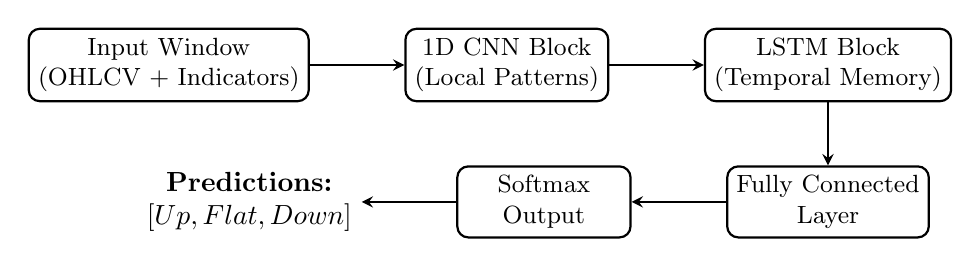
\begin{tikzpicture}[
    node distance=0.8cm and 1.2cm,
    box/.style={rectangle, draw, thick, align=center, rounded corners, minimum width=2.2cm, minimum height=0.75cm, font=\small},
    arrow/.style={->, thick, >=stealth}
]
\node[box] (input) {Input Window \\ (OHLCV + Indicators)};
\node[box, right=of input] (cnn) {1D CNN Block \\ (Local Patterns)};
\node[box, right=of cnn] (lstm) {LSTM Block \\ (Temporal Memory)};
\node[box, below=of lstm] (fc) {Fully Connected \\ Layer};
\node[box, left=of fc] (softmax) {Softmax \\ Output};
\node[align=center, left=of softmax] (output) {\textbf{Predictions:}\\ $[Up, Flat, Down]$};
\draw[arrow] (input) -- (cnn);
\draw[arrow] (cnn) -- (lstm);
\draw[arrow] (lstm) -- (fc);
\draw[arrow] (fc) -- (softmax);
\draw[arrow] (softmax) -- (output);
\end{tikzpicture}
}
\caption{Architecture of the proposed hybrid CNN--LSTM model.}
\label{fig:architecture}
\end{figure}

\section{Background \& Related Work}
The foundation for directional financial prediction using deep learning was established by
\citet{fischer2018deep}, who demonstrated that LSTMs consistently outperform memory-free models on
equity markets, though their sub-period analysis revealed profitability degradation across distinct
market eras. \citet{nelson2017stock} further validated the use of LSTMs specifically for predicting
asset price movements using standard technical indicators. Subsequent research successfully adapted
these methods to the cryptocurrency domain; \citet{zhao2021deep} utilized LSTMs on trade data to
achieve predictive accuracy high enough to be monetizable, while \citet{ghosh2020forecasting} validated
the standard use of logistic regression and random forests as robust financial baselines. Expanding on
sequence modeling, \citet{guo2021mrclstm} proposed a hybrid CNN--LSTM framework for Bitcoin, proving
that combining a CNN's local feature extraction with an LSTM's temporal memory significantly
outperforms either architecture in isolation. Our project builds on this lineage, using the hybrid
structure of \citet{guo2021mrclstm} to investigate the structural decay hinted at by
\citet{fischer2018deep}.

\section{Data Processing}
We will source high-frequency OHLCV (open, high, low, close, volume) data for BTC and ETH using the
public Binance API (\texttt{/api/v3/klines}). To enrich the feature space, we will compute standard
technical indicators such as RSI, MACD, and Bollinger Bands. To strictly prevent look-ahead bias, all
features will be normalized using z-scores calculated exclusively from the training-set distribution.
The continuous data will be sequenced into sliding windows of approximately 96 hours. Most importantly,
to support our core hypothesis regarding market regime shift, the dataset will be partitioned
chronologically into distinct, volatility-defined market phases (e.g., low-volatility consolidation
versus high-volatility drawdowns) rather than randomized splits, ensuring a rigorous test of
cross-regime generalization.

\section{Architecture}
The proposed model processes a sliding window of historical cryptocurrency data, forming an input
tensor of size $T \times F$, where $T$ represents the time-steps (e.g., 96 hours) and $F$ represents
the features. This sequence is first fed into a 1D~CNN block with ReLU activations to extract rich
local temporal patterns from short-term price movements. Crucially, the CNN preserves the temporal
sequence without condensing it. The LSTM then reads that enriched sequence in order, carrying memory
forward, and condenses all timesteps into a single summary vector that retains temporal dependencies.
Finally, this summary vector is routed through a fully connected output layer applying a softmax
activation to yield probabilities for the three directional classes: up, flat, and down. The
architecture will be implemented in PyTorch, using cross-entropy loss and the Adam optimizer, with
hidden dimensions tuned empirically on a validation set.

\section{Baseline Models}
To contextualize the deep learning model's performance, we will implement two non-sequential baselines.
The first is a naive momentum heuristic that predicts the direction of the most recent time-step. The
second is a logistic regression model, implemented via scikit-learn, trained on the same engineered
feature set. These memory-free baselines quantify the specific predictive value added by the
CNN--LSTM's temporal modeling.

\section{Ethical Considerations}
Financial machine learning models carry substantial ethical risks, particularly for retail
participants who face extreme volatility and potential catastrophic loss. Models that show high
backtest accuracy frequently collapse in production due to distribution shifts, creating a false sense
of security that misleads investors and amplifies market harm. By explicitly designing this project to
measure how a model's predictive edge degrades across market regimes, we address the imperative of
honest evaluation and highlight the dangers of deploying brittle, overfitted systems in real financial
environments without cross-regime stress-testing.

\bibliographystyle{plainnat}
\bibliography{refs}

\end{document}
